\section{Experiment}

\subsection{Determination of capacitance C of the capacitor component(RC circuit)}
dfsdlkfj

\begin{figure}[H]
	\centering
	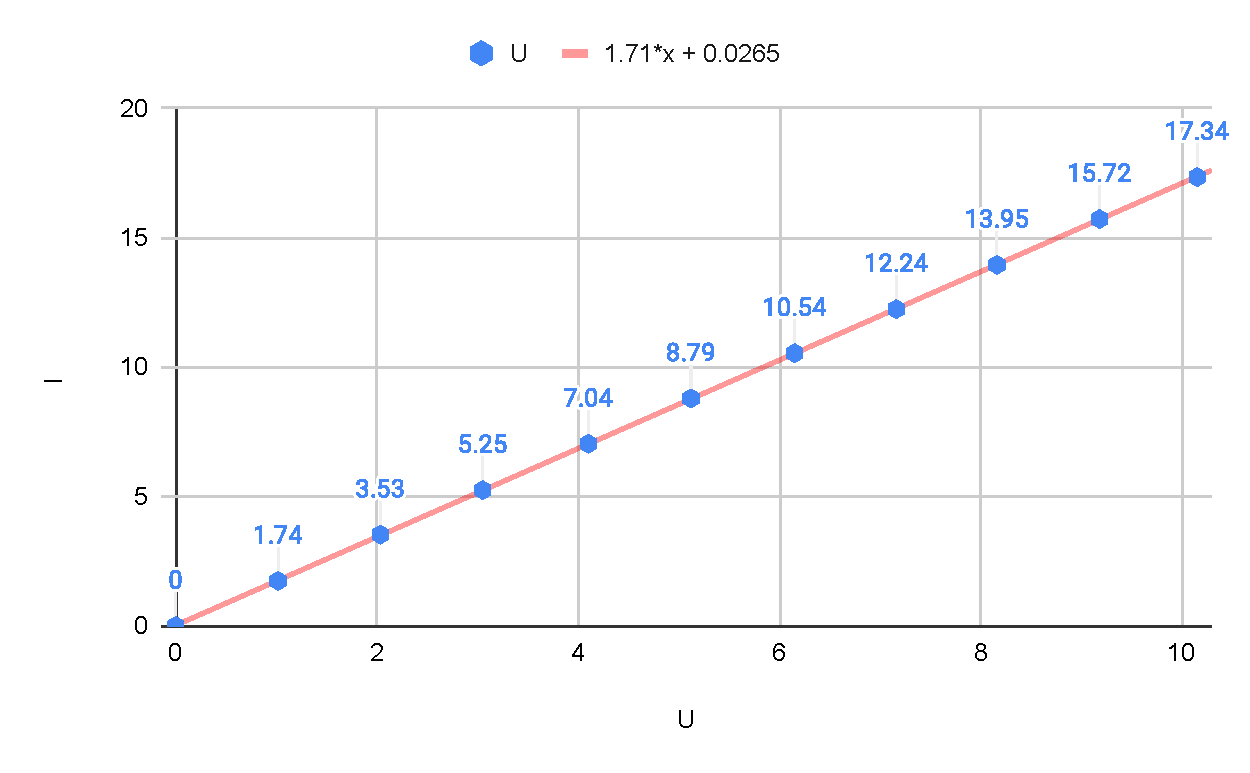
\includegraphics[width=14cm]{schematics/capacitor.pdf}
	\caption{RC circuit measurements }
	\label{fig:capacitance}
\end{figure}

\begin{table}[!ht]
    \centering
    \begin{tabular}{l|l|l}

         V & $U \SI{}{\volt}$ & $I \SI{}{\milli\ampere}$ \\ \hline
        0 & 0 & 0 \\ 
        100 & 1.017 & 1.74 \\ 
        200 & 2.034 & 3.53 \\ 
        300 & 3.051 & 5.25 \\ 
        400 & 4.1 & 7.04 \\ 
        500 & 5.12 & 8.79 \\ 
        600 & 6.15 & 10.54 \\ 
        700 & 7.16 & 12.24 \\ 
        800 & 8.16 & 13.95 \\ 
        900 & 9.18 & 15.72 \\ 
        1000 & 10.15 & 17.34 \\ 
    \end{tabular}
    \caption{RC circuit. f = \SI{300}{\hertz}} R = \SI{220}{\ohm} $Z_c$ = \SI{1.71}{\kilo\ohm}
    \label{tab:capacitance}
\end{table}

\subsubsection*{Calculations}

\begin{equation}
C = \frac{1}{2\pi f \sqrt{(Z_c^2 - R^2)}} =
 \frac{1}{2\pi 300 \sqrt{(1.71^2 - 220^2)}} =
 0.000000411562347
\end{equation}






\subsection{Determination of the inductance L of the inductor component (RL circuit)}

\begin{figure}[H]
	\centering
	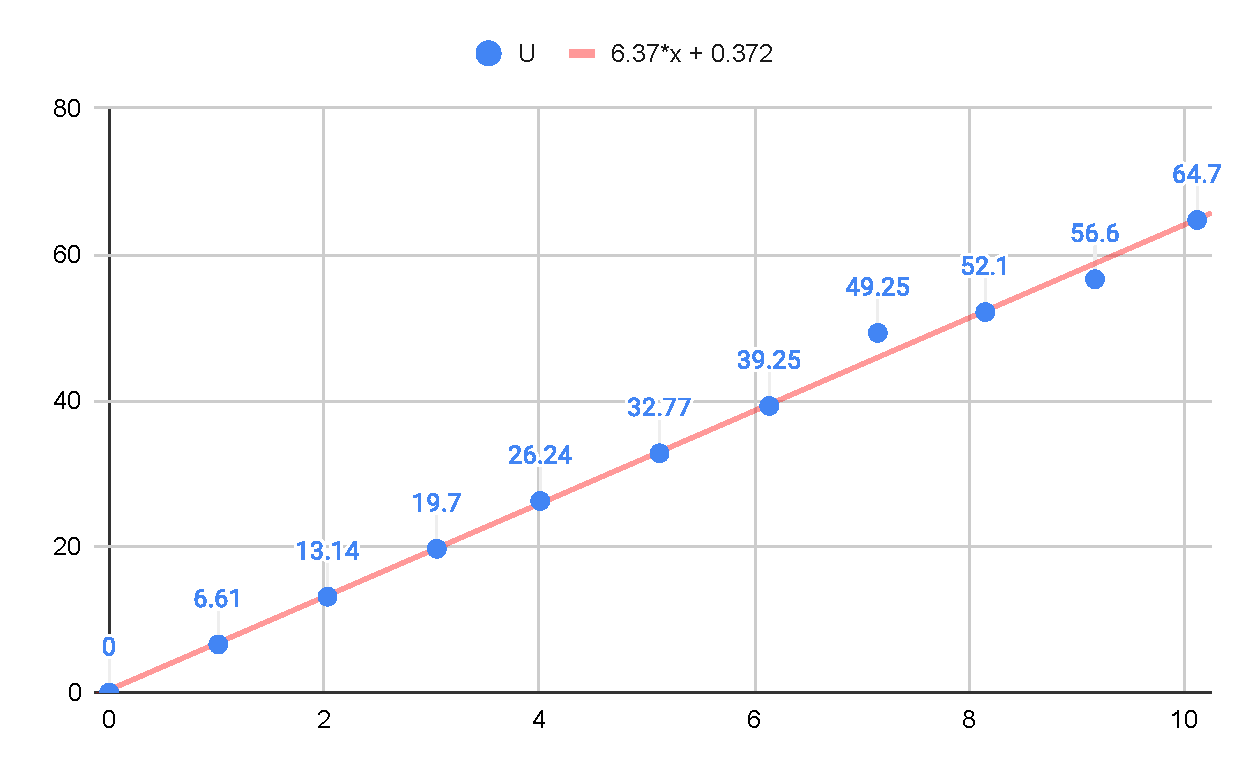
\includegraphics[width=14cm]{schematics/inductor.pdf}
	\caption{RC circuit measurements }
	\label{fig:inductance}
\end{figure}


\begin{table}[!ht]
    \centering
    \begin{tabular}{l|l|l}
        Vrsm & $U \SI{}{\volt}$ & $I \SI{}{\milli\ampere}$ \\ \hline
        0 & 0 & 0 \\ 
        100 & 6.61 & 1.016 \\ 
        200 & 13.14 & 2.032 \\ 
        300 & 19.7 & 3.048 \\ 
        400 & 26.24 & 4.01 \\ 
        500 & 32.77 & 5.12 \\ 
        600 & 39.25 & 6.14 \\ 
        700 & 49.25 & 7.15 \\ 
        800 & 52.1 & 8.15 \\ 
        900 & 56.6 & 9.17 \\ 
        1000 & 64.7 & 10.12 \\ 
    \end{tabular}
    \caption{RL circuit.f = \SI{300}{\hertz}} R = \SI{220}{\ohm} $R_l = \SI{0.6}{\ohm}$ $Z_c$ = \SI{6.37}{\kilo\ohm}
    \label{tab:capacitance}\end{table}

\subsubsection*{Calculations}

\begin{equation}
	L = \frac{\sqrt{Z_L^2-(R+R_L)^2}}{2\pi f} = 
	\frac{\sqrt{6370^2-(220+0.6)^2}}{2\pi 300} =
	1.333838664
\end{equation}



\subsection{Verification of the Ohm's Law for the alternation current (RLC circuit)}

\begin{figure}[H]
	\centering
	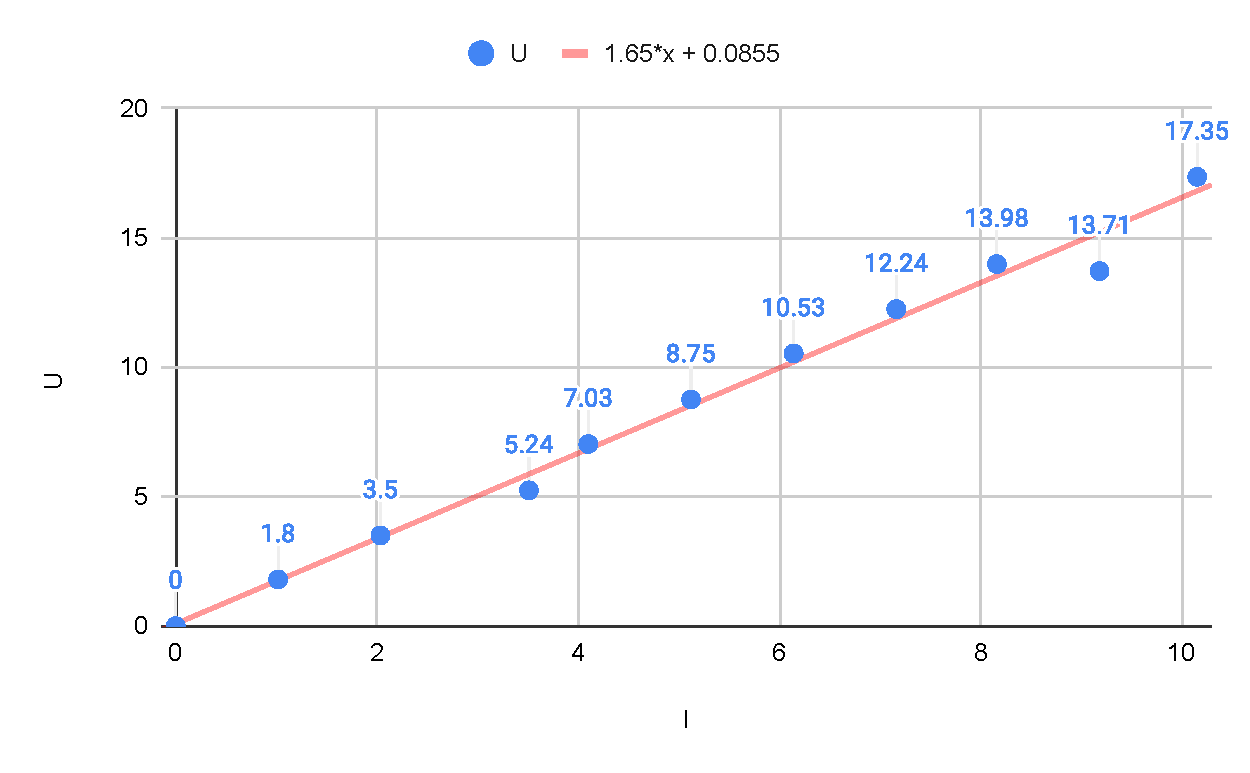
\includegraphics[width= 14cm]{schematics/verification.pdf}
	\caption{RC circuit measurements }
	\label{fig:verification}
\end{figure}

\begin{table}[!ht]
    \centering
    \begin{tabular}{l|l|l}
        Vrsm & U & I \\ \hline
        0 & 0 & 0 \\ 
        100 & 1.8 & 1.017 \\ 
        200 & 3.5 & 2.034 \\ 
        300 & 5.24 & 3.51 \\ 
        400 & 7.03 & 4.1 \\ 
        500 & 8.75 & 5.12 \\ 
        600 & 10.53 & 6.14 \\ 
        700 & 12.24 & 7.16 \\ 
        800 & 13.98 & 8.16 \\ 
        900 & 13.71 & 9.18 \\ 
        1000 & 17.35 & 10.15 \\ 
    \end{tabular}
    \caption{RCL circuit.f = \SI{300}{\hertz}} R = \SI{220}{\ohm} $R_l = \SI{0.6}{\ohm}$ $Z_{cl}$ = \SI{1.65}{\kilo\ohm}
    \label{tab:verification}
    \end{table}
    
    \subsubsection*{Calculations}
\begin{multline}
	Z_2 = \sqrt{(R+R_L)^2 + \left(\left(2 \pi f L\right) - \left(\frac{1}{2 \pi f C}\right)\right)^2} = \\
	\sqrt{(220+0.6)^2 + \left(\left(2 \pi 300 \times 1.333838664\right) - \left(\frac{1}{2 \pi 300 \times 0.000000411562347}\right)\right)^2}= \\
	1244.89743
\end{multline}
    


\subsection*{Formulas used in the calculations}


\begin{equation}
C = \frac{1}{2\pi f \sqrt{(Z_c^2 - R^2)}}
\end{equation}

\begin{equation}
	L = \frac{\sqrt{Z_L^2-(R+R_L)^2}}{2\pi f}
\end{equation}

\begin{equation}
	Z_2 = \sqrt{(R+R_L)^2 + \left(\left(2 \pi f L\right) - \left(\frac{1}{2 \pi f C}\right)\right)^2}
\end{equation}
